\documentclass[conference,compsoc,11pt]{IEEEtran}

\usepackage{multirow}
\usepackage{amsmath}
\usepackage{dsfont}

\usepackage[style=verbose]{biblatex}
\addbibresource{./bibliography.bib}

% *** CITATION PACKAGES ***
%
%\ifCLASSOPTIONcompsoc
%  \usepackage[nocompress]{cite}
%\else
%  \usepackage{cite}
%\fi

% *** GRAPHICS RELATED PACKAGES ***
%
\ifCLASSINFOpdf
\else
\fi

%\hyphenation{op-tical net-works semi-conduc-tor}
\usepackage{graphicx}
\graphicspath{ {../misc/report_material/} }

\begin{document}
\title{Time Series Classification
\\ \large Artificial Neural Networks and Deep Learning -- A.Y. 2022/2023}

\author{\IEEEauthorblockN{Paolo Botta\IEEEauthorrefmark{1},
Teo Bucci\IEEEauthorrefmark{2} and Silvia Caresana\IEEEauthorrefmark{3}}
\IEEEauthorblockA{M.Sc. Mathematical Engineering,
Politecnico di Milano - Milan, Italy\\
Email: \IEEEauthorrefmark{1}paolo.botta@mail.polimi.it,
\IEEEauthorrefmark{2}teo.bucci@mail.polimi.it,
\IEEEauthorrefmark{3}silvia.caresana@mail.polimi.it\\
Student ID: \IEEEauthorrefmark{1}10612869,
\IEEEauthorrefmark{2}10621873,
\IEEEauthorrefmark{3}10630163\\
Codalab Group: ``Just3Neurons''}
}
\maketitle

%\begin{abstract}
%TODO%In this report, we explore and compare the development process we had to design a Convolutional Neural Network able to classify 14 different plants species through their leaves images as input.
%\end{abstract}

\IEEEpeerreviewmaketitle

\section{Introduction}
The given dataset consists of $2429$ samples with $6$ features each, where every feature is a time series of $T = 36$ steps. Every sample belongs to one of the 12 different classes.

The task suggests to use Categorical Cross-Entropy as loss function. If $y_{ij}$ is the output probability of class $j$ for observation $i$, then:
\begin{equation*}
\operatorname{Loss}(y_{\text{pred}},y_{\text{true}}) = - \frac{1}{N} \sum_{i=1}^N \sum_{j=1}^J y_{\text{true},ij} \log(y_{\text{pred},ij})
\end{equation*}
where $N$ is the number of samples and $J = 12$ is the number of classes.

As metric we used Accuracy as requested:
\begin{equation*}
\operatorname{Accuracy} = \frac{1}{N} \sum_{i=1}^N \mathds{1}_{[\operatorname{argmax}_j (y_{\text{pred},ij}) = \operatorname{argmax}_j (y_{\text{true},ij})]}
\end{equation*}

In addition, we also considered the F1--score per class to better understand the weaknesses of the model.

The dataset was split according to an 85:15 train-validation ratio and the results of this report are the ones we obtained on the validation set.

We started tackling the problem building different models and comparing their performances. Finally, based on the accuracy score and the F1--scores we selected the best performing one.

\section{Data Pipeline}

\subsection{Pre-Processing}

For a better modelling of the data we chose to apply a standardization. Since the different features span very different value ranges (see Figure \ref{fig:features}), we normalized with respect to them by subtracting the mean and dividing by the standard deviation.
The same transformation was saved and then applied on the validation and remote test set.

\begin{figure}[h!]
\centering
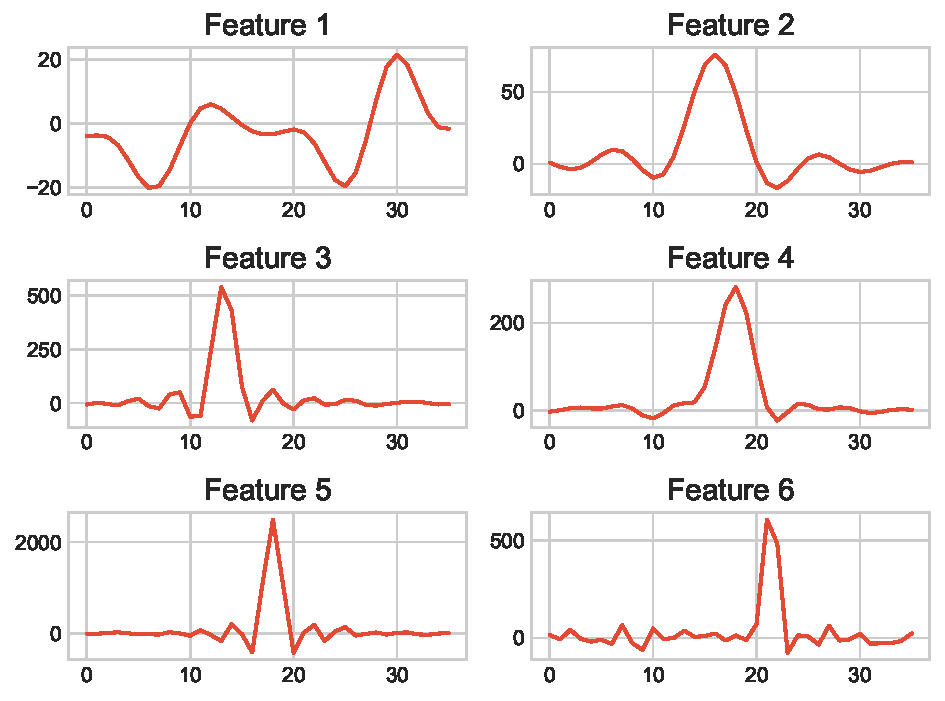
\includegraphics[width=2.5in]{datum_5.pdf}
\caption{Plot of the 6 features from a random sample of the original dataset across time.}
\label{fig:features}
\end{figure}

\subsection{Data Augmentation}

We were a bit reluctant to use data augmentation in this case, not knowing the underlying meaning of the features. Nevertheless we considered some transformations\footcite{Iwana_2021} as can be seen in Figure \ref{fig:augmentation}. After some trials, we kept \textbf{Scaling} and \textbf{Permutation}, since the others were either too computationally intensive or deteriorated too much the data.
%\begin{itemize}
%    \item Jittering
%    \item Scaling
%    \item Permutation
%    \item Window Slicing
%    \item Time Warp
%\end{itemize}

\begin{figure}[h!]
\centering
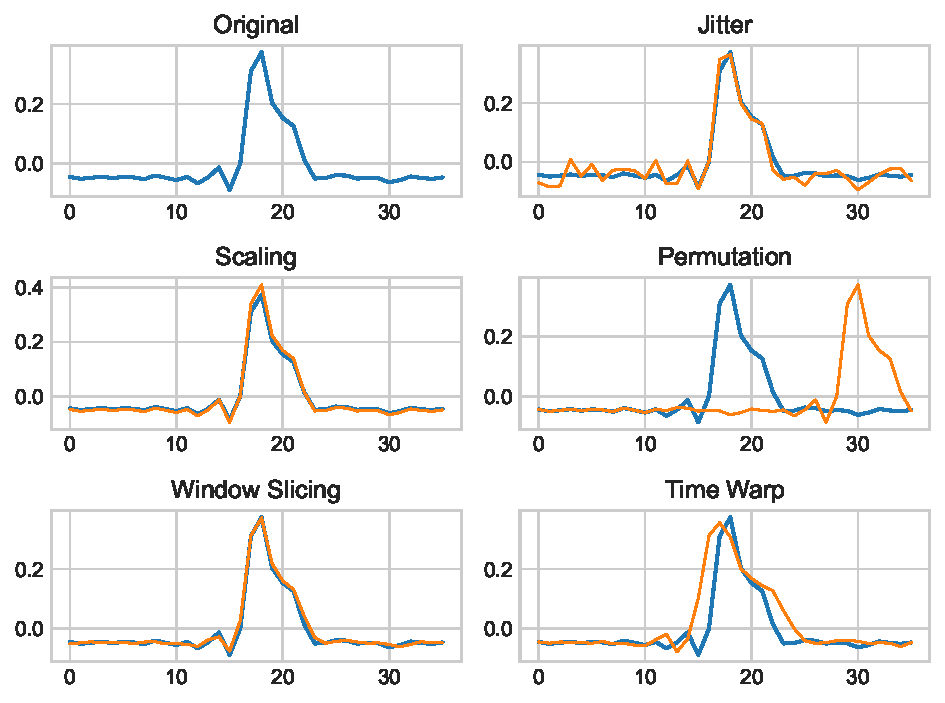
\includegraphics[width=3.1in]{augmentation_vis.pdf}
\caption{Examples of the different augmentations we explored. This example shows feature 4 from a random sample from the standardized dataset.}
\label{fig:augmentation}
\end{figure}

\section{Models}

In the following models the \texttt{Dropout} rate was always set to $0.5$.
%All the considered models were create by varying the features extractor, followed by \texttt{Dense} and \texttt{Dropout} layers, with a rate of $0.5$.

\subsection{Vanilla LSTM}\label{sec:features-extractor}

\begin{center}
\begin{tabular}{c}
\hline
LSTM(128) (x2)\\
Dropout\\
Dense(128)\\
\hline
\end{tabular}
\end{center}

\subsection{Bidirectional LSTM}

\begin{center}
\begin{tabular}{c}
\hline
BidirectionalLSTM(128) (x2)\\
Dropout\\
Dense(128)\\
\hline
\end{tabular}
\end{center}

\subsection{1D CNN}

\begin{center}
\begin{tabular}{c}
\hline
Conv1D + MaxPooling1D (x4)\\
GlobalAveragePooling1D\\
Dropout\\
Dense(512)\\
Dropout\\
Dense(256)\\
\hline
\end{tabular}
\end{center}

\subsection{Keras tuner}

After having an initial idea of the potential of the previous models, we turned to the Keras tuner, allowing it to explore different configurations in terms of \texttt{LSTM}, \texttt{Conv1D} and \texttt{Dense} layers. We used the Bayesian Optimization tuner for a maximum of 30 trials.

\begin{center}
\begin{tabular}{c}
\hline
Conv1D (x3)\\
BidirectionalLSTM(256)\\
GlobalAveragePooling1D\\
Dropout\\
Dense(128)\\
BatchNormalization\\
Dropout\\
\hline
\end{tabular}
\end{center}

\subsection{Inception Time}

\textbf{Inception Time}\footcite{Del2020Time} is a model based on Convolutional Neural Networks. It consists of a series of \textbf{Inception Modules} followed by a GAP Layer and a Fully Connected one (in our case 2 \texttt{Dense} layer with 256 and 128 units). Moreover, a residual connection is added at every third inception module in order to mitigate the vanishing gradient problem. The Inception Module (see Figure \ref{fig:inception-module}) consists of 4 layers:
\begin{itemize}
    \item Bottleneck Layer that reduces the dimensionality and improves generalization;
    \item Parallel Convolutional Layers of different size acting on the same input feature map;
    \item MaxPooling that improves the invariance to small perturbation;
    \item Depth Concatenation Layer that concatenates the output of convolutions and MaxPooling.
\end{itemize}

\begin{figure}[h!]
\centering
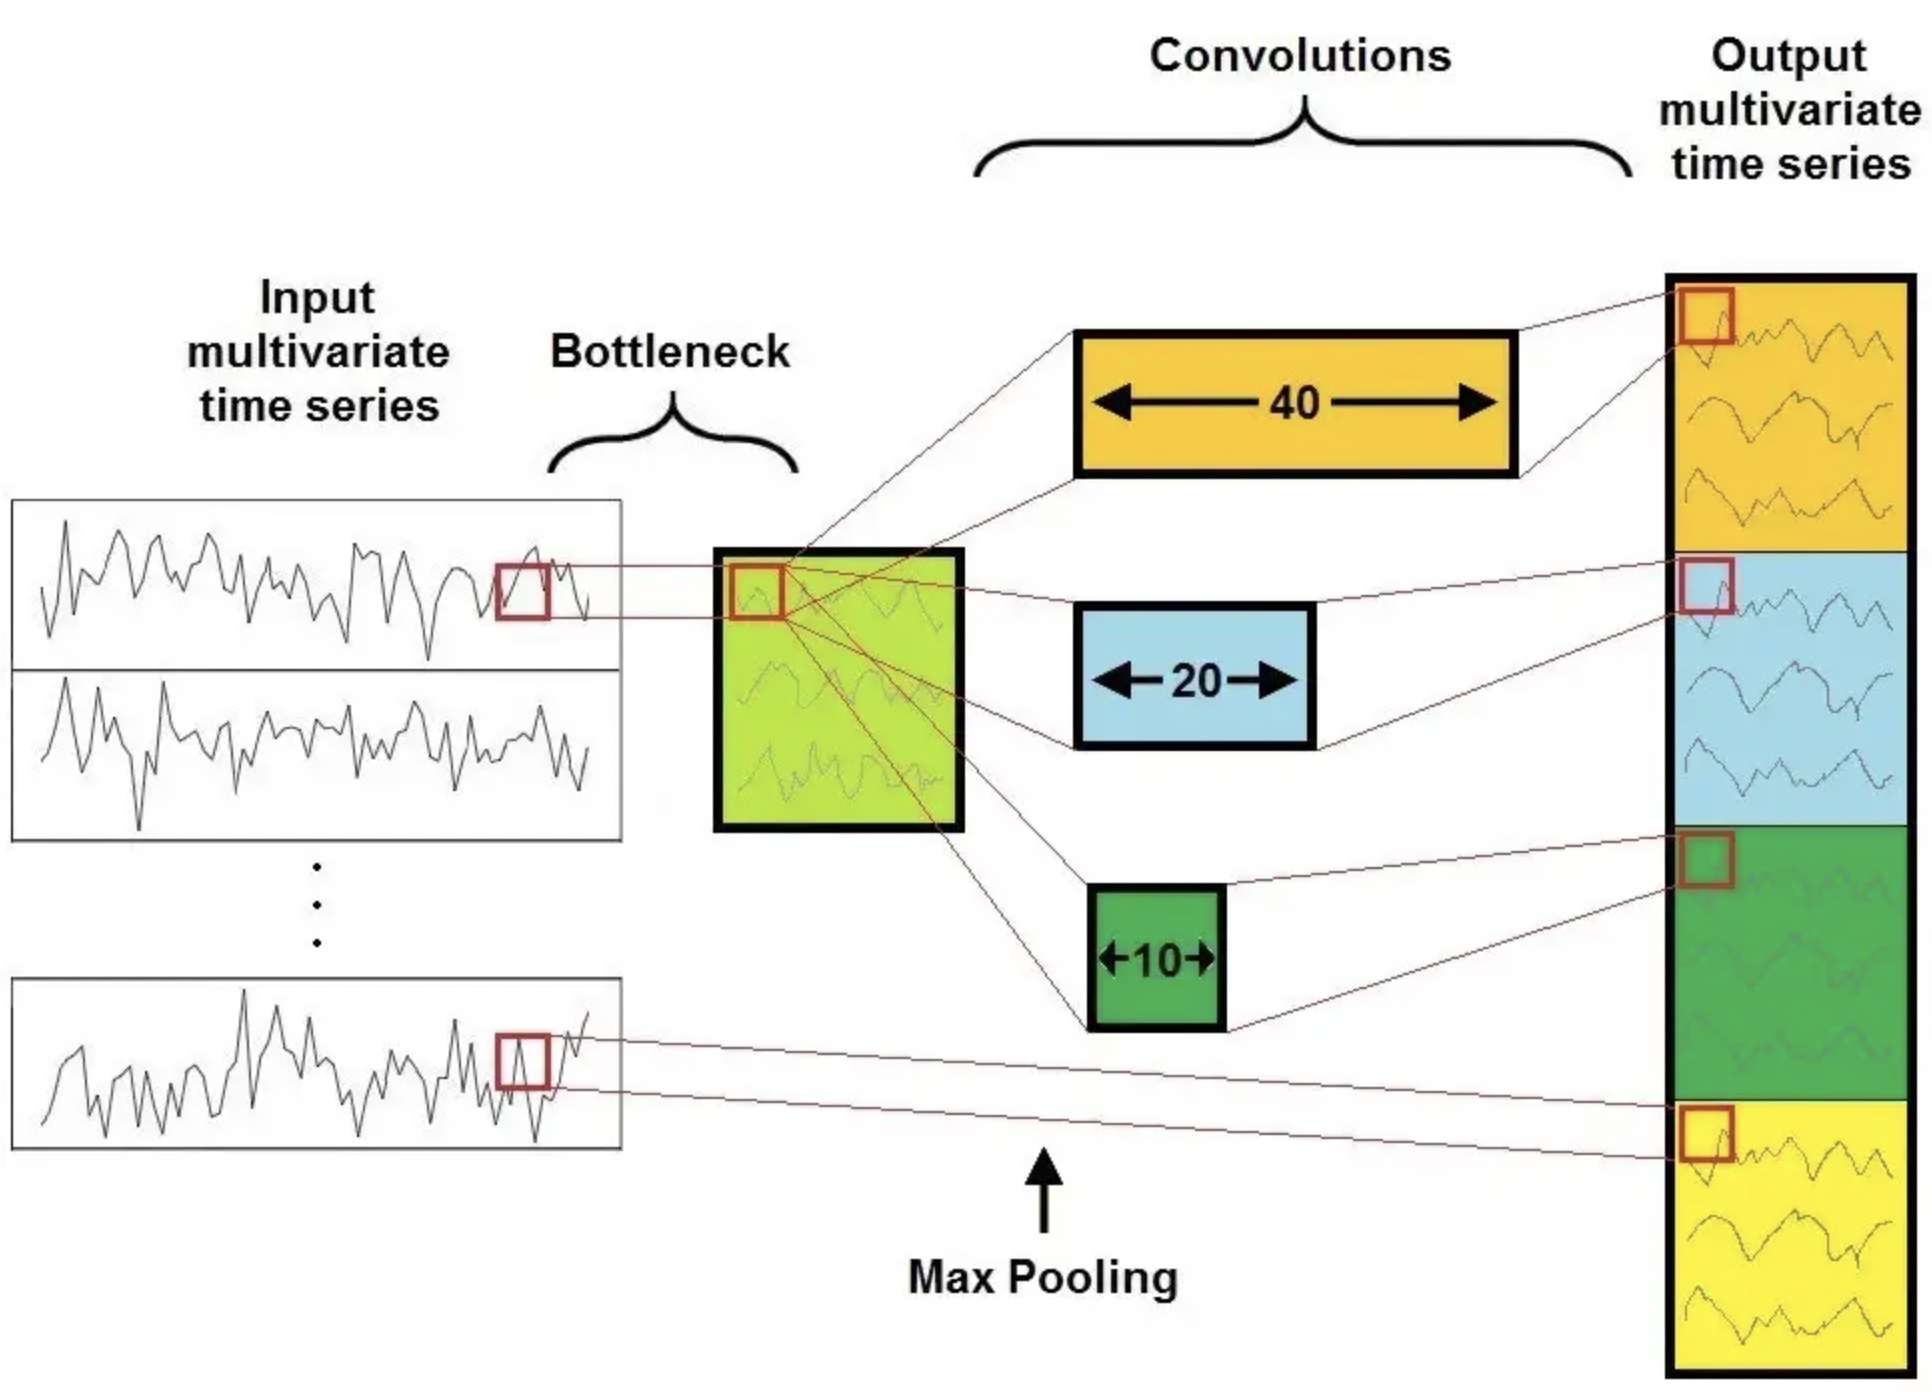
\includegraphics[width=2.6in]{inception_module.png}
\caption{Inception module.}
\label{fig:inception-module}
\end{figure}

\section{Training techniques}

In terms of training, we used for all models:
\begin{itemize}
    \item Batch size: 16
    \item Optimizer: Adam
    \item Learning rate: 0.001
    \item Callbacks: \textbf{EarlyStopping} with patience 20, \textbf{ReduceLROnPlateau} with patience 5 and factor 0.5
\end{itemize}

\subsection{Class imbalance}\label{sec:cl_imb}

Class imbalance played an important role, as can be seen in Figure \ref{fig:imbalance}.

\begin{figure}[h!]
\centering
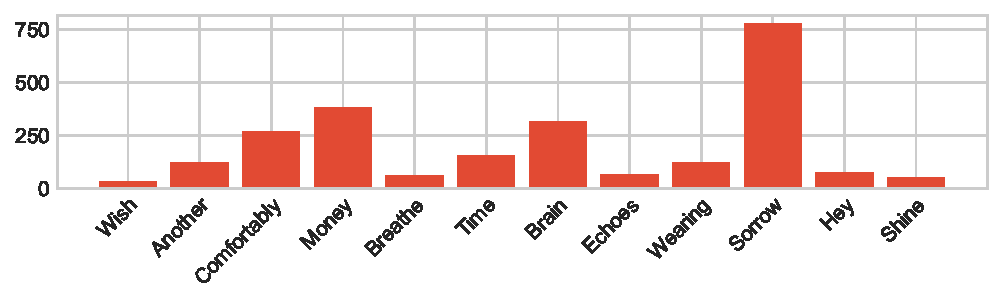
\includegraphics[width=3.1in]{class_imbalance.pdf}
\caption{Number of samples in each class.}
\label{fig:imbalance}
\end{figure}

The approach we followed was to train 12 different Inception models, each one very strong in classifying a single class. To do so, each time we gave weight 10 to the class in consideration and weight 1 to all the others. Finally, these models were put in an ensemble, together with the base Inception, by taking the simple average.

\section{Model choice}\label{sec:model-choice}

We compared the different models, both with and without augmentation (except the Keras tuner, which was too computationally intensive to run with augmentation too). Even though augmentation improved the accuracy in almost all cases, this didn't happen with the final Inception of Section \ref{sec:cl_imb}. However, without augmentation it outperformed all the others by 4\%. Therefore, that is the final model we choose.

\begin{center}
\begin{tabular}{ l c c }
\hline\hline
 & Std. & Std. + Aug.\\
\hline
Vanilla LSTM       & 66.30\% & 68.77\% \\
Bidirectional LSTM & 69.59\% & 74.79\% \\
1D CNN             & 73.42\% & 74.52\% \\
Keras tuner        & 74.52\% & - \\
Inception Time     & 74.52\% & 76.16\% \\
Inception Ensemble & \textbf{80.55\%} & 76.99\% \\
\hline\hline
\end{tabular}
\end{center}

\section{Conclusion}

\subsection{Performance}

The results of the final model both on the train, the validation and the remote test set are as follows:

\begin{center}
\begin{tabular}{ l c c }
\hline\hline
Train acc.  & Val acc.  & Test acc. \\
\hline
95.74\%     & 80.55\%   & 74.00\% \\
\hline\hline
\end{tabular}
\end{center}

\noindent The F1--scores are:

\begin{center}
\footnotesize
\setlength\tabcolsep{2pt}
%\bgroup
%\def\arraystretch{0.5}%  1 is the default, change whatever you need
\begin{tabular}{l|cccccccccccc}
\hline
%Wish & Another & Comfortably & Money & Breathe & Time & Brain & Echoes & Wearing & Sorrow & Hey & Shine \\
Class & 0 & 1 & 2 & 3 & 4 & 5 & 6 & 7 & 8 & 9 & 10 & 11 \\
F1 & 1 & 0.67 & 0.99 & 0.65 & 0 & 0.67 & 0.90 & 0.50 & 0.97 & 0.82 & 1 & 0.59 \\
\hline
\end{tabular}
%\egroup
\end{center}

% con 4 cifre significative
% 1 & 0.6667 & 0.9882 & 0.6549 & 0 & 0.6667
% 0.902 & 0.5 & 0.9677 & 0.8218 & 1 & 0.5882 \\

\noindent The final confusion matrix can be seen in Figure \ref{fig:confusion}.

\begin{figure}[h!]
\centering
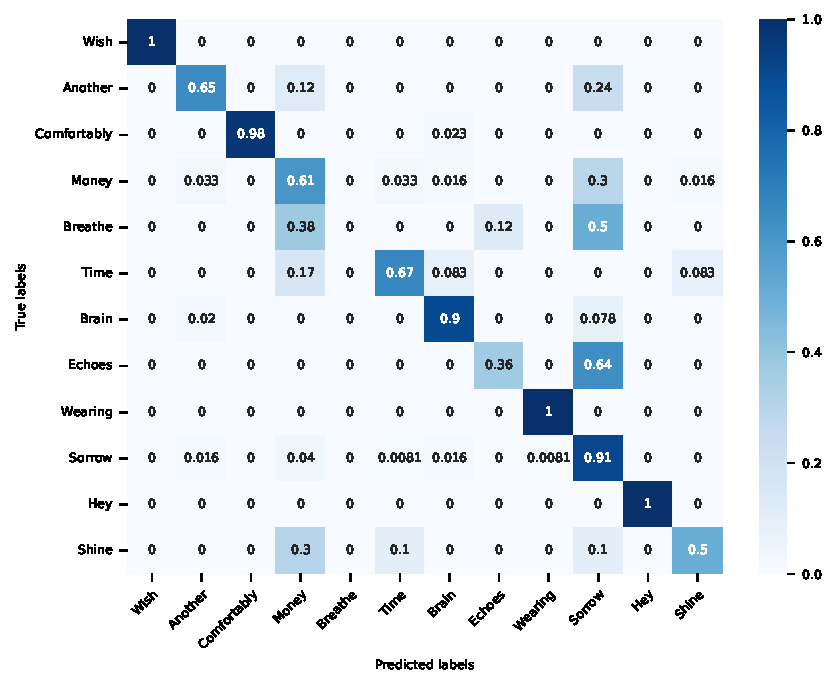
\includegraphics[width=3.1in]{confusion_crazy_ensemble.pdf}
\caption{Normalized confusion matrix of the final model.}
\label{fig:confusion}
\end{figure}

\subsection{Further Developments}

A few aspects of our work might use some improvement. We could do some more preliminary analysis on the dataset to understand more suitable preprocessing steps.

Moreover, we are not yet satisfied with how we dealt with class imbalance, specifically because class \texttt{Breathe} got an F1--score of 0 in almost all models, except the one obtained with the Keras tuner. This deserves some attention.

Speaking of attention, we quickly tried using \texttt{Attention} layers, but we weren't quite used to them and didn't manage to reach results as good as with the classical techniques. Therefore, we sticked to those for the time being, but we're sure that some improvements can be made from the architecture side.

%\begin{thebibliography}{1}
%\bibitem{IEEEhowto:perez}
%L. Perez and J. Wang}, \emph{The Effectiveness %of Data Augmentation in Image Classification %using Deep Learning} - \relax Stanford %University, 2017.
%\end{thebibliography}

\end{document}